\section{Используемые технологии} 
\label{sec:practice:technology_used}
Выбор технологий является важным предварительным этапом разработки сложных информационных систем. Платформа и язык программирования, на котором будет реализована система, заслуживает большого внимания, так как исследования показали, что выбор языка программирования влияет на производительность труда программистов и качество создаваемого ими кода ~\cite{mcconnell_2005}.

Ниже перечислены некоторые факторы, повлиявшие на выбор технологий:
\begin{itemize}
  \item Среди различных языков программирования разработчик имеет наибольший опыть в PHP;
  \item Разработчик имеет опыт работы с объектно-ориентированными языками программирования, и решениями в полной мере реализующие возможности ООП;
  \item Платформа Symfony хорошо подходит для реализации серверной бизнес - логики приложения, и разработчик имеет опыт работы с этой платформой.
\end{itemize}


\subsection{Язык программирования PHP}
\label{sub:practice:php_overview}
PHP - скриптовый язык общего назначения, интенсивно применяемый для разработки веб-приложений. В настоящее время поддерживается подавляющим большинством хостинг-провайдеров и является одним из лидеров среди языков, применяющихся для создания динамических веб-сайтов~\cite{php_documents}.

Главная область применения PHP - написание скриптов, работающих на стороне сервера; таким образом, PHP способен выполнять все то, что выполняет любая другая программа CGI, например, обрабатывать данные форм, генерировать динамические страницы или отсылать и принимать cookies. Но PHP способен выполнять намного больше.

PHP доступен для большинства операционных систем, включая Linux, многие модификации Unix (такие как HP-UX, Solaris и OpenBSD), Microsoft Windows, Mac OS X, RISC OS, и многие другие. Также в PHP включена поддержка большинства современных веб-серверов, таких как Apache, IIS и многих других. Подойдет любой веб-сервер, способный использовать бинарный файл FastCGI PHP, например, lighttpd или nginx. PHP может работать в качестве модуля или функционировать в качестве процессора CGI.

Таким образом, выбирая PHP, вы получаете свободу выбора операционной системы и веб-сервера. Более того, у вас появляется выбор между использованием процедурного или объектно-ориентированного программирования (ООП) или же их сочетания.

PHP способен генерировать не только HTML. Доступно формирование изображений, файлов PDF и даже роликов Flash (с использованием libswf и Ming), создаваемых «на лету». PHP также способен генерировать любые текстовые данные, такие, как XHTML и другие XML-файлы. PHP может осуществлять автоматическую генерацию таких файлов и сохранять их в файловой системе вашего сервера вместо того, чтобы отдавать клиенту, организуя, таким образом, серверный кэш для вашего динамического контента.

Одно из преимуществ язка PHP - поддержка широкого круга баз данных. Для создания сценария использующего базу данных можно воспользоваться расширением, специфичным для отдельной базы данных (таким как mysql) или использовать уровень абстракции от базы данных, такой как PDO, или подсоединиться к любой базе данных, поддерживающей Открытый Стандарт Соединения Баз Данных (ODBC), с помощью одноименного расширения ODBC. Для других баз данных, таких как CouchDB, можно воспользоваться cURL или сокетами~\cite{php_documents}.

PHP также поддерживает «общение» с другими сервисами через такие протоколы, как LDAP, IMAP, SNMP, NNTP, POP3, HTTP, COM (на платформах Windows) и многих других. Кроме того, вы получаете возможность работать с сетевыми сокетами напрямую. PHP поддерживает стандарт обмена сложными структурами данных WDDX практически между всеми языками веб-программирования. Обращая внимание на взаимодействие между различными языками, следует упомянуть о поддержке объектов Java и возможности их использования в качестве объектов PHP.

PHP имеет много возможностей по обработке текста, включая регулярные выражения Perl (PCRE) и много других расширений и инструментов для обработки и доступа к XML документам. В PHP обработка XML-документов стандартизирована и происходит на базе мощной библиотеки lib-xml2, расширив возможности обработки XML добавлением новых расширений SimpleXML, XMLReader и XMLWriter~\cite{php_documents}.

\subsubsection{Область применения }
\label{sub:practice:whereis_php}
В области веб-программирования, в частности серверной части, PHP - один из популярных сценарных языков (наряду с JSP, Perl и языками, используемыми в ASP.NET).

Популярность в области построения веб-сайтов определяется наличием большого набора встроенных средств для разработки веб-приложений. 

Основные из них:
\begin{itemize}
  \item автоматическое извлечение POST и GET-параметров, а также переменных окружения веб-сервера в предопределённые массивы;
  \item взаимодействие с большим количеством различных систем управления базами данных, такми как: MySQL,  SQLite, PostgreSQL, Oracle, ODBC и др;
  \item автоматизированная отправка HTTP-заголовков;
  \item работа с HTTP-авторизацией;
  \item работа с локальными и удалёнными файлами, сокетами;
  \item обработка файлов, загружаемых на сервер;
  \item работа с cookies и сессиями.
\end{itemize}

В настоящее время PHP используется сотнями тысяч разработчиков. Согласно рейтингу корпорации TIOBE, базирующемся на данных поисковых систем, в мае 2016 года PHP находился на 6 месте среди языков программирования. К крупнейшим сайтам, использующим PHP, относятся Facebook, Wikipedia, Vkonakte, Badoo и др.



\subsubsection{Элементарные типы PHP }
\label{sub:practice:types_php}

РНР является слабо типизированным языком. Это означает, что нет необходимости объявлять тип данных, который должна хранить переменная. Так, в пределах одной и той же области видимости переменная \$number может содержать как значение 2, так и строку " two " ("два"). В строго типизированных языках программирования, таких как С или Java, вы обязаны определить тип переменной , прежде чем присваивать ей значение, и, конечно, это значение должно быть указанного типа. Но это не означает, что в РНР нет понятия типа. Каждое значение, которое можно присвоить переменной, имеет свой тип~\cite{zandstra_2015}.

Ниже представлены элементарные типы языка PHP:
\begin{itemize}
  \item Boolean - одно из двух значений true или false;
  \item Integer - целое число;
  \item Double - число с плавающей точкой;
  \item String - символьные данные(строка);
  \item Array - массив;
  \item Object - объект;
  \item Resource - дескриптор, используемый для идентификации и работы с внешними ресурсами , такими как базы данных или файлы; 
  \item Null - неинициализированное значение.
\end{itemize}


\subsubsection{Объектно-ориентированное программирование }
\label{sub:practice:oop_php}
Ключевое слово class было зарезервировано ещё в третьей версии языка. В четвёртой версии стало возможно создавать классы и объекты на их основе. Однако принципы ООП поддерживались лишь частично, так например, все члены (переменные и методы) были открыты. К тому же создание объектов было дорогой операцией и работали они медленно.

Начиная с пятой версии PHP обладает полной поддержкой ООП. Работа с классами была оптимизирована и теперь такой код работает достаточно быстро.

Класс в PHP объявляется с помощью ключевого слова class. Методы и поля класса могут быть общедоступными (public, по умолчанию), защищёнными (protected) и скрытыми (private). PHP поддерживает все три основных механизма ООП - инкапсуляцию, полиморфизм подтипов и наследование (родительский класс указывается с помощью ключевого слова extends после имени класса). Поддерживаются интерфейсы (ставятся в соответствие с помощью implements). Разрешается объявление финальных, абстрактных методов и классов. Множественное наследование классов не поддерживается, однако класс может реализовывать несколько интерфейсов. Для обращения к методам родительского класса используется ключевое слово parent.

Начиная с версии 5.4.0 множественное наследование может быть реализовано с помощью механизма трейтов. Повторное использование кода заключено в использовании кода трейта в нескольких классах. Допускается использовать в одном классе несколько трейтов. Механизм трейтов имеет средства разрешения конфликтов имён. При запуске программы код трейта будет «вкомпилирован» в код содержащего его класса.

Классы в PHP имеют ряд «магических» методов, начинающихся с двух символов подчёркивания. Особо стоит отметить конструктор (\_\_construct(), в версиях до 5.0 конструктором служил метод, одноимённый с классом) и деструктор (\_\_destruct()), а также методы чтения (\_\_get()) и записи (\_\_set()), свёртывания (\_\_sleep()) и развёртывания (\_\_wakeup()), клонирования (\_\_clone()) и др. Эти методы являются достаточно гибким инструментом: переопределяя их, можно добиться существенного изменения поведения объекта.

Экземпляры класса создаются с помощью ключевого слова new, обращение к полям и методам объекта производится с использованием оператора "->", для доступа к метода и свойствам объявленным с ключевым словом static используется оператор "::". Для доступа к членам класса из его методов используется переменная \$this.

Пример объектно-ориентированной конструкции на языке PHP: 
\begin{lstlisting}
          class C1 extends C2 implements I1, I2
          {
            private $a;
            protected $b;

            function __construct($a, $b)
            {
              parent::__construct($a, $b);
              $this->a = $a;
              $this->b = $b;
            }

            public function plus()
            {
              return $this->a + $this->b;
            }
          }

          $d = new C1(1, 2);
          echo $d->plus(); // 3
\end{lstlisting}

\subsubsection{Расширение возможностей ядра PHP }
\label{sub:practice:extebtions_php}
Интерпретатор состоит из ядра и подключаемых модулей, «расширений», представляющих собой динамические библиотеки. Расширения позволяют дополнить базовые возможности языка, предоставляя возможности для работы с базами данных, сокетами, динамической графикой, криптографическими библиотеками, документами формата PDF и тому подобным. Любой желающий может разработать своё собственное расширение и подключить его. Существует огромное количество расширений, как стандартных, так и созданных сторонними компаниями и энтузиастами, однако в стандартную поставку входит лишь несколько десятков хорошо зарекомендовавших себя. Множество расширений доступно в репозитории PECL.

Ниже представлены «расширения» языка использованные в этой дипломной работе:
\begin{itemize}
  \item mbstring - предоставляет функции для работы с многобайтными строками, которые облегчают работу c многобайтными кодировками в PHP. Кроме того, mbstring занимается конвертированием строк из одной кодировки в другую. mbstring предназначен для работы с Unicode-кодировками, такими, как UTF-8 и UCS-2, а также с многими однобайтными кодировками;
  \item xml - Данное расширение позволит вам создавать XML - анализаторы и далее определить обработчики для различных событий. Каждый XML-анализатор также имеет несколько параметров, которые вы можете настраивать. В работе требовалось для корректной работы с YAML файлами конфигураций платформы Symfony;
  \item pdo - определяет простой и согласованный интерфейс для доступа к базам данных в PHP.
\end{itemize}

\subsubsection{Режимы запуска интерпретатора }
\label{sub:practice:extebtions_php}

SAPI - это внешний уровень абстракции, предназначенный для встраивания интерпретатора в другие приложения и отвечает за его работу (запуск, остановка, передача скриптов на исполнение, доступ к внешним данным). Существует несколько основных SAPI определяющих способы запуска и использования PHP:

\begin{itemize}
    \item   В качестве модуля к веб-серверу (прим. Apache модуль mod\_php). В этом случае интерпретатор PHP выполняется в окружении процесса веб-сервера. Веб-сервер управляет количеством запущенных процессов PHP и сообщает им какие скрипты требуется исполнить;

    \item   CGI SAPI. Использование CGI подразумевает запуск нового процесса для обработки каждого запроса. Для исполнения PHP скрипта веб-сервер запускает ./php-cgi /path/to/script.php. Сам принцип такого использования подразумевает, что интерпретатор PHP исполняет только один скрипт, после чего заканчивает свою работу. Затраты на запуск процесса интерпретатора и его инициализацию очень часто сопоставимы или даже превышают затраты на исполнение PHP скрипта. Для решения этой проблемы в CGI SAPI был введен режим FastCGI. В этом режиме PHP интерпретатор запускается как независимый сервер, обрабатывающий входящие запросы на исполнение PHP скриптов по протоколу FastCGI, что позволяет ему работать с любым веб-сервером поддерживающим этот протокол~\cite{php_documents};

    \item   FPM SAPI, известный как php-fpm - это другая реализация протокола FastCGI. Создан изначально Андреем Нигматулиным как отдельный патч для использования в социальной сети Badoo. Данная реализация решала ряд проблем, которые мешали использованию CGI/FastCGI SAPI. В частности, появилась возможность перезапуска пула интерпретаторов PHP без потери запросов, запуск нескольких пулов под разными пользователями, аварийный перезапуск интерпретаторов в случае проблем с ними и ещё несколько приятных дополнений. В дальнейшем над патчем работали несколько человек, был добавлен режим динамического управления числом запущенных процессов PHP (по принципу управления числом процессов в веб-сервере Apache), и начиная с версии PHP 5.3.3 php-fpm был включен в PHP как отдельное SAPI;

    \item   В качестве скрипта командной строки (CLI SAPI), являющегося исполняемым файлом, который вызывается пользователем из командной строки; скрипт выполняется в окружении вызвавшего пользователя. В этом случае возможно использование PHP для создания клиентских GUI-приложений и решения административных задач в операционных системах UNIX, Linux, Microsoft Windows, Mac OS X и AmigaOS. Однако в таком качестве он не получил распространение, отдавая первенства Perl, Python и VBScript.
    Начиная с версии PHP 5.4.0 в CLI SAPI появилась возможность запуска PHP как отдельного HTTP сервера. Однако этот режим предназначен исключительно для разработки, так как запускает только один процесс интерпретатора и выполняет все запросы исключительно последовательно~\cite{php_documents}.
\end{itemize}

\subsection{ORM Doctrine}
\label{sub:practice:doctrine}
Doctrine - объектно-реляционный проектор (ORM) для PHP 5, который базируется на слое абстракции доступа к БД (DBAL). Одной из ключевых возможностей Doctrine является запись запросов к БД на собственном объектно-ориентированном диалекте SQL, называемый DQL (Doctrine Query Language) и базирующийся на идеях HQL (Hibernate Query Language).

Средства ORM Doctrine позволяют генерировать классы описывающие таблицы базы данных автоматически, если таблицы уже описаны на уровне базы данных. Но если таблицы не были созданы можно описать сущность и сгенерировать таблицы в базе данных на основе описания класса и его полей. Описывать структуру таблицы можно посредством использования XML, YAML, PHP нотаций, или же использовать аннотации прямо в классе описывающем таблицу. 

Пример описания сущности описывающей таблицу в базе данных посредством аннотаций:
\begin{lstlisting}
          /**
           * @ORM\Entity(
                  repositoryClass="AppBundle\Repository\TaskGroupRepository"
           )
           */
          class TaskGroup
          {
              /**
               * @var integer
               *
               * @ORM\Column(name="id", type="integer")
               * @ORM\Id
               * @ORM\GeneratedValue(strategy="AUTO")
               */
              private $id;

              /**
               * @ORM\OneToMany(
                      targetEntity="AppBundle\Entity\Task",
                      mappedBy="group",
                      cascade={"persist"}
                  )
               */
              private $tasks;

              /**
               * @var string
               *
               * @ORM\Column(
                      name="description",
                      type="string",
                      length=30,
                      nullable=false
                  )
               */
              private $description;

              /**
               * @ORM\ManyToOne(
                      targetEntity="User",
                      inversedBy="taskGroups"
                  )
               */
              private $user;

              public function __construct()
              {
                  $this->tasks = new ArrayCollection();
              }
          }
\end{lstlisting}

Данное описание позволяет создать в БД таблицу с  полями id(INT 11), description(VARCHAR 30) и user\_id(INT 11). Благодаря использоованию аннотации ManyToOne над полем user и установки обратной связи в описании сущности User, колонка user\_id таблицы task\_groups в БД будет асоциирована с колонкой id таблицы users.

\begin{lstlisting}
          /**
           *
           * @ORM\OneToMany(targetEntity="AppBundle\Entity\TaskGroup", mappedBy="user")
           */
          private $taskGroups;
\end{lstlisting}

Благодаря такой связи на уровне ORM, в БД будет создана таблица task\_groups со связью Many-To-One к таблице users.

\begin{figure}[ht]
\centering
  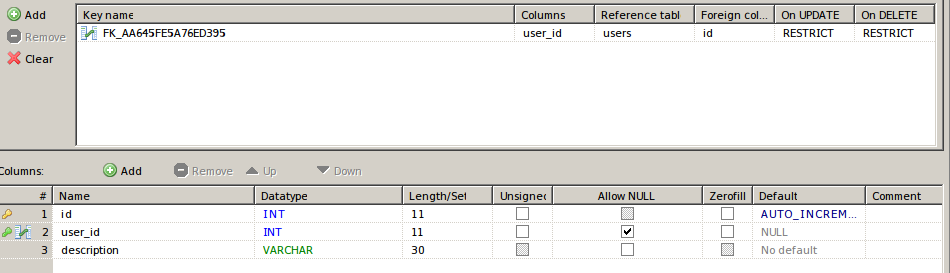
\includegraphics[scale=0.4]{images/table_tg.png}  
  \caption{  Созданная таблица в БД }
  \label{fig:domain:symfony_request_workflow}
\end{figure}

Данный подход позволяет добится аналогичного поведения сущностей на уровне PHP кода с поведением табилц в базе данных. Что в последствии помогает разработчику отказатся от использования SQL-конструкции при разработке веб-приложеиня. 

Doctrine cледует паттерну Data mapper. Для создания пользователя может использоватся следующий код:

\begin{lstlisting}
          $user = new User();
          $user->setName("john");
          $user->setPassword("doe");
          $entityManager->persist($user);
          $entityManager->flush();
          echo "The user with id " . $user->getId() . "has been saved.";
\end{lstlisting}


Получение оъекта класса Product соответствующего строке в базе данных по уникальному \$id:
\begin{lstlisting}
          $em = $this->getDoctrine();
          $product = $em->getRepository('AcmeStoreBundle:Product')->find($id);
\end{lstlisting}

Добавление оъекта класса Product с именем 'Name' в базу данных:
\begin{lstlisting}
          $product = new Product();
          $product->setName('Name');
          $em = $this->getDoctrine()->getManager();
          $em->persist($product);
          $em->flush();
\end{lstlisting}

Одной из особенностей Doctrine является низкий уровень конфигурации, необходимый для запуска проекта. Doctrine может генерировать классы объектов из существующей базы данных, и программист может затем указать отношения и добавить пользовательские функциональные возможности к сгенерированным классам. Нет необходимости создавать или поддерживать сложные схемы базы данных XML, как это видно во многих других платформах.

Еще одной важной особенностью Doctrine является возможность произвольной записи запросов базы данных в диалекте OO (объектно - ориентированный) SQL, называемом DQL (Doctrine Query Language), который был разработан на основе  HQL Hibernate. Класс QueryBuilder позволяет создавать запросы через свободный интерфесы. Эти интерфейсы предоставляют разработчикам мощные альтернативы SQL, которые поддерживают гибкость и позволяют переключать базы данных, не требуя дублирования кода.

Ниже представлен пример испольования QueryBuilder в Doctrine:
\begin{lstlisting}
          $repository = $this->getDoctrine()->getRepository('AppBundle::Product');
          $query = $repository
                      ->createQueryBuilder('p')
                      ->where('p.price>:price')
                      ->setParameter('price','19.99')
                      ->orderBy('p.price','ASC')
                      ->getQuery();
          $products = $query->getResult();
\end{lstlisting}

Явное написание запросов к БД не всегда необходимо, так как Doctrine выполняет объединения и выбирает связанные объекты автоматически. Малые проекты можно построить не используя запросы.

\subsection{Обработчик шаблонов Twig}

Twig — компилирующий обработчик шаблонов с открытым исходным кодом, написанный на языке программирования PHP. Армин Ронахер написал Twig в 2008 году для платформы блогов Chyrp. Он больше не возвращался к разработке и в большей степени занимался разработкой на Python. Синтаксис языка шаблонов Twig берёт начало от движков шаблонов Jinja и Django, первый из которых также создан Ронахером. Идею данного шаблонизатора развивает и поддерживает Фабьен Потенсье, ведущий разработчик и идеолог фреймворка Symfony, в котором Twig используется по умолчанию.

\subsection{Платформа Symfony}
\label{sub:practice:symfony}

Symfony - свободная программная платформа, написанная на PHP, который использует паттерн Model-View-Controller.

Symfony предлагает быструю разработку и управление веб-приложениями, позволяет легко решать рутинные задачи веб-программиста. Работает только с PHP 5 и выше. Имеет поддержку множества баз данных (MySQL, PostgreSQL, SQLite или любая другая PDO-совместимая СУБД). Информация о реляционной базе данных в проекте должна быть связана с объектной моделью. Это можно сделать при помощи ORM инструмента. В Symfony это Doctrine.

Symfony бесплатен и публикуется под лицензией MIT.

\subsubsection{Реализация паттерна MVC на примере Symfony }

Концепция MVC (Model-View-Controller: модель-вид-контроллер) часто упоминается в мире веб программирования. Каждый, кто хоть как-то связан с разработкой веб приложений, так или иначе сталкивался с данной аббревиатурой. 

MVC предназначен для разделения бизнес-логики и пользовательского интерфейса, чтобы разработчики могли легко изменять отдельные части приложения, не затрагивая другие. В архитектуре MVC модель предоставляет данные и правила бизнес-логики, представление отвечает за пользовательский интерфейс (например, текст, поля ввода), а контроллер обеспечивает взаимодействие между моделью и представлением.

При работе с платформой Symfony в качестве модели можно использовать сущность построенную средствами ORM Doctrine. В качестве вида можно использовать шаблон написанный средствами обработчика шаблона Twig. А контроллер представляет из себя обычный класс включающий в себя методы для обработки конкретных запросов.

\begin{lstlisting}
          public function getTask(Task $task = null)
          {
              if ($task) {
                  /**@var User $user */
                  $user = $this->container->get('security.token_storage')
                  ->getToken()->getUser();
                  $userRepo = $this->getDoctrine()->getManager()
                                  ->getRepository(User::class);
                  /**@var UserRepository $userRepo */
                  $taskCreator = $userRepo->getTaskCreatorUser($task);
                  if ($taskCreator->getId() === $user->getId()) {
                      $taskResponseGenerator = $this
                          ->get('app.task_response_arr_generator');
                      return new PrettyJsonResponse(
                          ['response' => true] + 
                          $taskResponseGenerator->generateTaskResponse($task),
                          200);
                  } else {
                      return new PrettyJsonResponse([
                          'response' => true,
                          'error' => 'Not Allowed for this user!'
                      ], 401);
                  }
              } else {
                  return new PrettyJsonResponse([
                      'response' => true,
                      'error' => 'Task not found!'
                  ], 404);
              }
          }
\end{lstlisting}
Данный пример пытается получить экземпляры сущности описанной классом Task из БД, и в случае успеха возвращает клиенту данные конвертированные в JSON объект. 

\subsubsection{Схема обработки запроса Symfony }
Традиционная схема обработки запроса платформы Symfony выглядит следующим образом:
\begin{figure}[ht]
\centering
  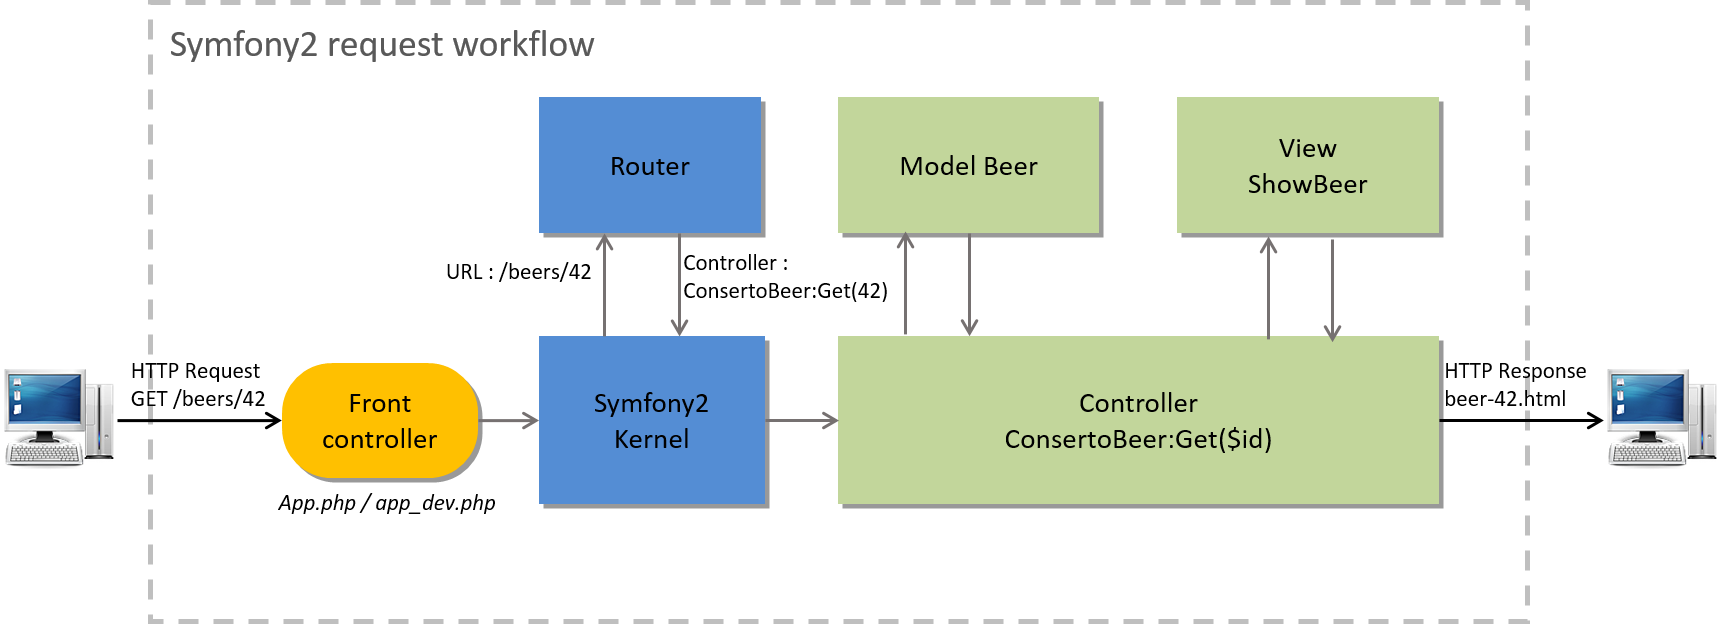
\includegraphics[scale=0.35]{images/request-workflow.png}  
  \caption{  Схема обработки запроса Symfony }
  \label{fig:domain:symfony_request_workflow}
\end{figure}

На данной диаграмме продемонстрированна  реализация архитектуры «клиент-сервер». В начале жизненного цикла обработки клиентского запроса, представленного в виде HTTP-запроса отправленного посредством браузера, сервер перенаправляет входные параметры  на серверный компонент «Контроллер входа». Данный компонент ответственен за обработку входных параметров прим.(GET и POST параметры).

После обработки входных параметров «Контроллер входа» передает управление ядру платформы, который в свою очередь обращается к компоненту «Router» для определения метода класса «контроллера» ответственного за обработку данного запроса. Если метод «контроллера» ответственный за обработку данного типа запроса найден, то жизненный цикл перенаправляется к нему. 

Далее на основе логики в методе класса «контроллера» генерируется ответ на запрос клиента. В данном случае ответ представляет из себя HTML-документ. Данная логиика может быть представлена в виде обращения к БД, либо каких-либо сложных вычислений основаннных на пользовательских данных для динамической генерации страницы, или же возвращать статические данные.
 
\begin{figure}[ht]
\centering
  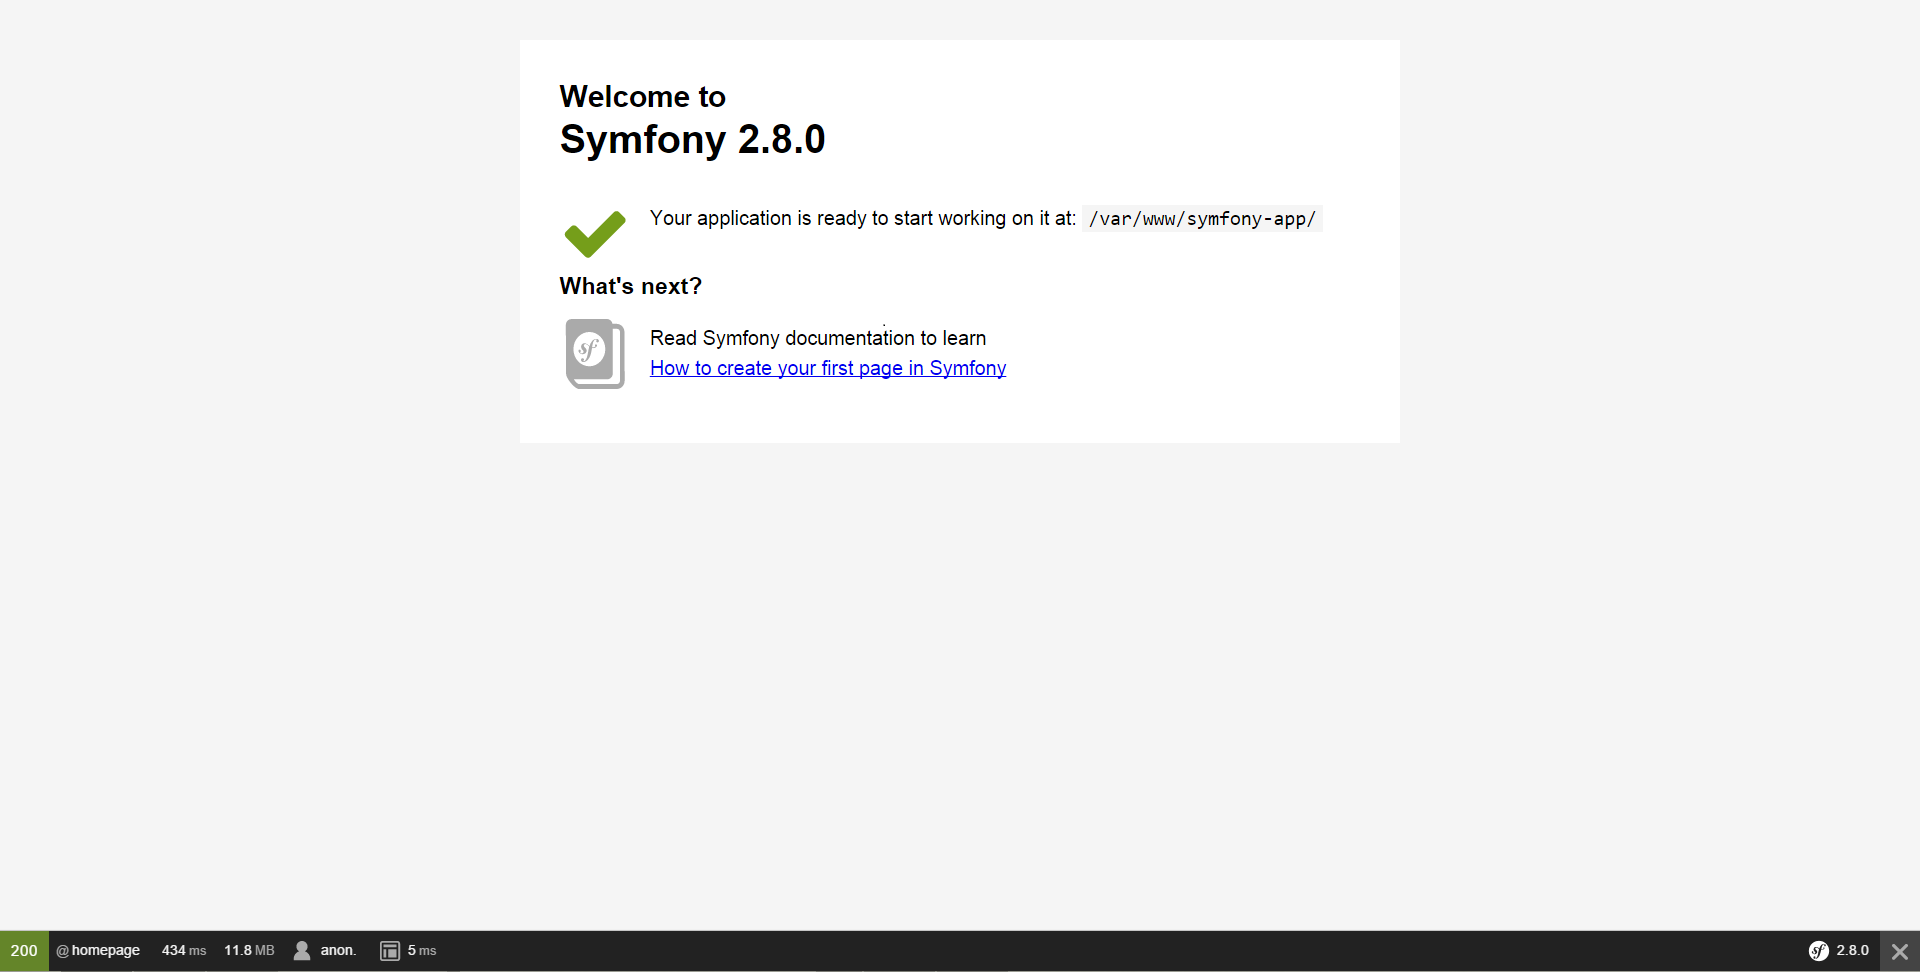
\includegraphics[scale=0.3]{images/welcome.png}  
  \caption{  Пример ответа от сервера в виде статической HTML страницы }
  \label{fig:domain:symfony_request_workflow}
\end{figure}

Если же компонент «Router» не находит метода класса «контроллера» ответственного за обработку данного запроса, и платформа работает в режиме разработки, то будет возвращён HTML документ с подробным описанием проблемы. 


Данный ответ состоит из:

\begin{itemize}
  \item подробного сообщения об ошибке;
  \item строки кода в которой произошла эта ошибка и была сгенерирована исключительная ситуация;
  \item названия класса описывающего исключительные ситуации данного типа;
  \item цепочки вызовов методов. 
\end{itemize}


\begin{figure}[hb]
\centering
  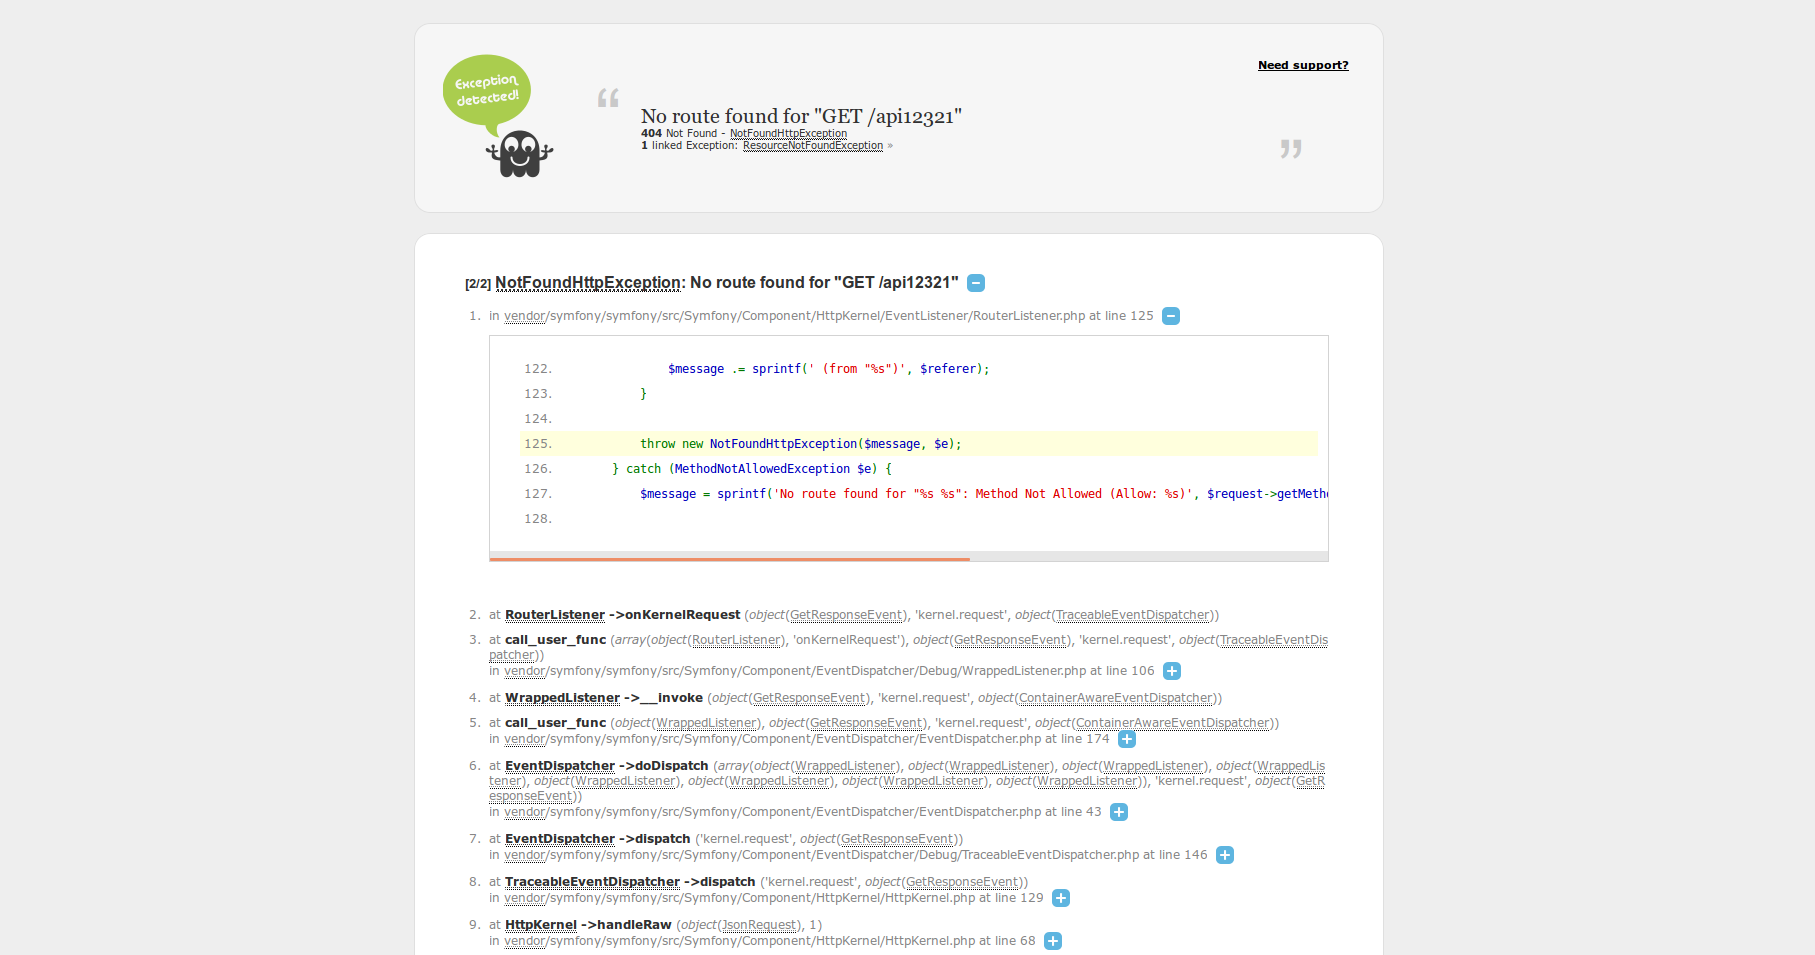
\includegraphics[scale=0.2]{images/symfony_exception.png}  
  \caption{  Пример ответа от сервера при котором произошла ислючительная ситуация }
  \label{fig:domain:symfony_request_workflow}
\end{figure}

\subsection{Система автоматизации развертывания Docker}
Docker — программное обеспечение для автоматизации развёртывания и управления приложениями в среде виртуализации на уровне операционной системы. Позволяет «упаковать» приложение со всем его окружением и зависимостями в контейнер, который может быть перенесён на любую Linux-систему с поддержкой cgroups в ядре, а также предоставляет среду по управлению контейнерами. 

Программное обеспечение функционирует в среде Linux с ядром, поддерживающим cgroups и изоляцию пространств имён (namespaces). Для экономии дискового пространства проект использует файловую систему Aufs с поддержкой технологии каскадно-объединённого монтирования: контейнеры используют образ базовой операционной системы, а изменения записываются в отдельную область. Также поддерживается размещение контейнеров в файловой системе Btrfs с включённым режимом копирования при записи.

В состав программных средств входит демон — сервер контейнеров (запускается командой docker -d), клиентские средства, позволяющие из интерфейса командной строки управлять образами и контейнерами, а также API, позволяющий в стиле REST управлять контейнерами программно.

Демон обеспечивает полную изоляцию запускаемых на узле контейнеров на уровне файловой системы (у каждого контейнера собственная корневая файловая система), на уровне процессов (процессы имеют доступ только к собственной файловой системе контейнера, а ресурсы разделены средствами libcontainer), на уровне сети (каждый контейнер имеет доступ только к привязанному к нему сетевому пространству имён и соответствующим виртуальным сетевым интерфейсам).

Набор клиентских средств позволяет запускать процессы в новых контейнерах (docker run), останавливать и запускать контейнеры (docker stop и docker start), приостанавливать и возобновлять процессы в контейнерах (docker pause и docker unpause). Серия команд позволяет осуществлять мониторинг запущенных процессов (docker ps по аналогии с ps в Unix-системах, docker top по аналогии с top и другие). Новые образы возможно создавать из специального сценарного файла (docker build, файл сценария носит название dockerfile), возможно записать все изменения, сделанные в контейнере в новый образ (docker commit). Все команды могут работать как с docker-демоном локальной системы, так и с любым сервером Docker, доступным по сети. Кроме того, в интерфейсе командной строки встроены возможности по взаимодействию с публичным репозиторием Docker Hub, в котором размещены предварительно собранные образы контейнеров, например, команда docker search позволяет осуществить поиск образов среди размещённых в нём, образы можно скачивать в локальную систему (docker pull), возможно также отправить локально собранные образы в Docker Hub (docker push).
